\cleardoublepage
\chapter{Hardware}\label{chap:hardware}
% To do: 
% Color Scheme
% Red - Not started
% Yellow - In progress
% Blue - Done, under approval
% Green - Done and approved
\todo[inline,color=red!40]{*Latter add Section for the actuator}
\todo[inline,color=red!40]{*Chapter Introduction}

\todo[inline,color=yellow!40]{*1 - Selection}
\todo[inline,color=blue!40]{ a) Microphone}
\todo[inline,color=blue!40]{ b) Accelerometer}
\todo[inline,color=blue!40]{ c) Piezoelectric}
\todo[inline,color=blue!40]{ d) Microcontroller}
\todo[inline,color=blue!40]{ e) Solenoid}

\todo[inline,color=yellow!40]{*2 - Design}
\todo[inline,color=red!40]{ a) Accelerometer}
\todo[inline,color=blue!40]{ b) Piezoelectric}
\todo[inline,color=blue!40]{ c) Solenoid}

\todo[inline,color=blue!40]{*3 - Capture/Coupling}
\todo[inline,color=blue!40]{ a) Microphone}
\todo[inline,color=blue!40]{ b) Accelerometer}
\todo[inline,color=blue!40]{ c) Piezoelectric}
%% Writing %%%%%%%%%%%%%%%%%%%%%%%%%%%%%%%%%%%%%%%%%%%%%%%%%%%%%%%%%%%%
\section{Selection}
\subsection{Microphone}
With the interest of understanding what is the system response to an external stimulation, it is needed a simple method to record that response.  The easy way to do that is by using a microphone to capture the sound produced, when hitting the side surface of the LPG bottle, by the time the study of this started due to the fact there wasn’t available the proper material for it, in the case a microphone and a soundboard, lead to search for an alternative for it.

Although there are various alternatives for it, like the embedded computer microphone, or an external microphone, none of those were able to properly capture the sound and be mounted in a practical setup, the alternative for this solution is recurring to the use of the microphone of a regular phone.  The phone itself is connected via USB to the computer, on which additional software was installed to allow access in real time to the data captured by the microphone of the phone.  In figure 4.1 is an illustration of the connection between the microphone of the phone and the computer.
\begin{figure}[]
    \centering
    %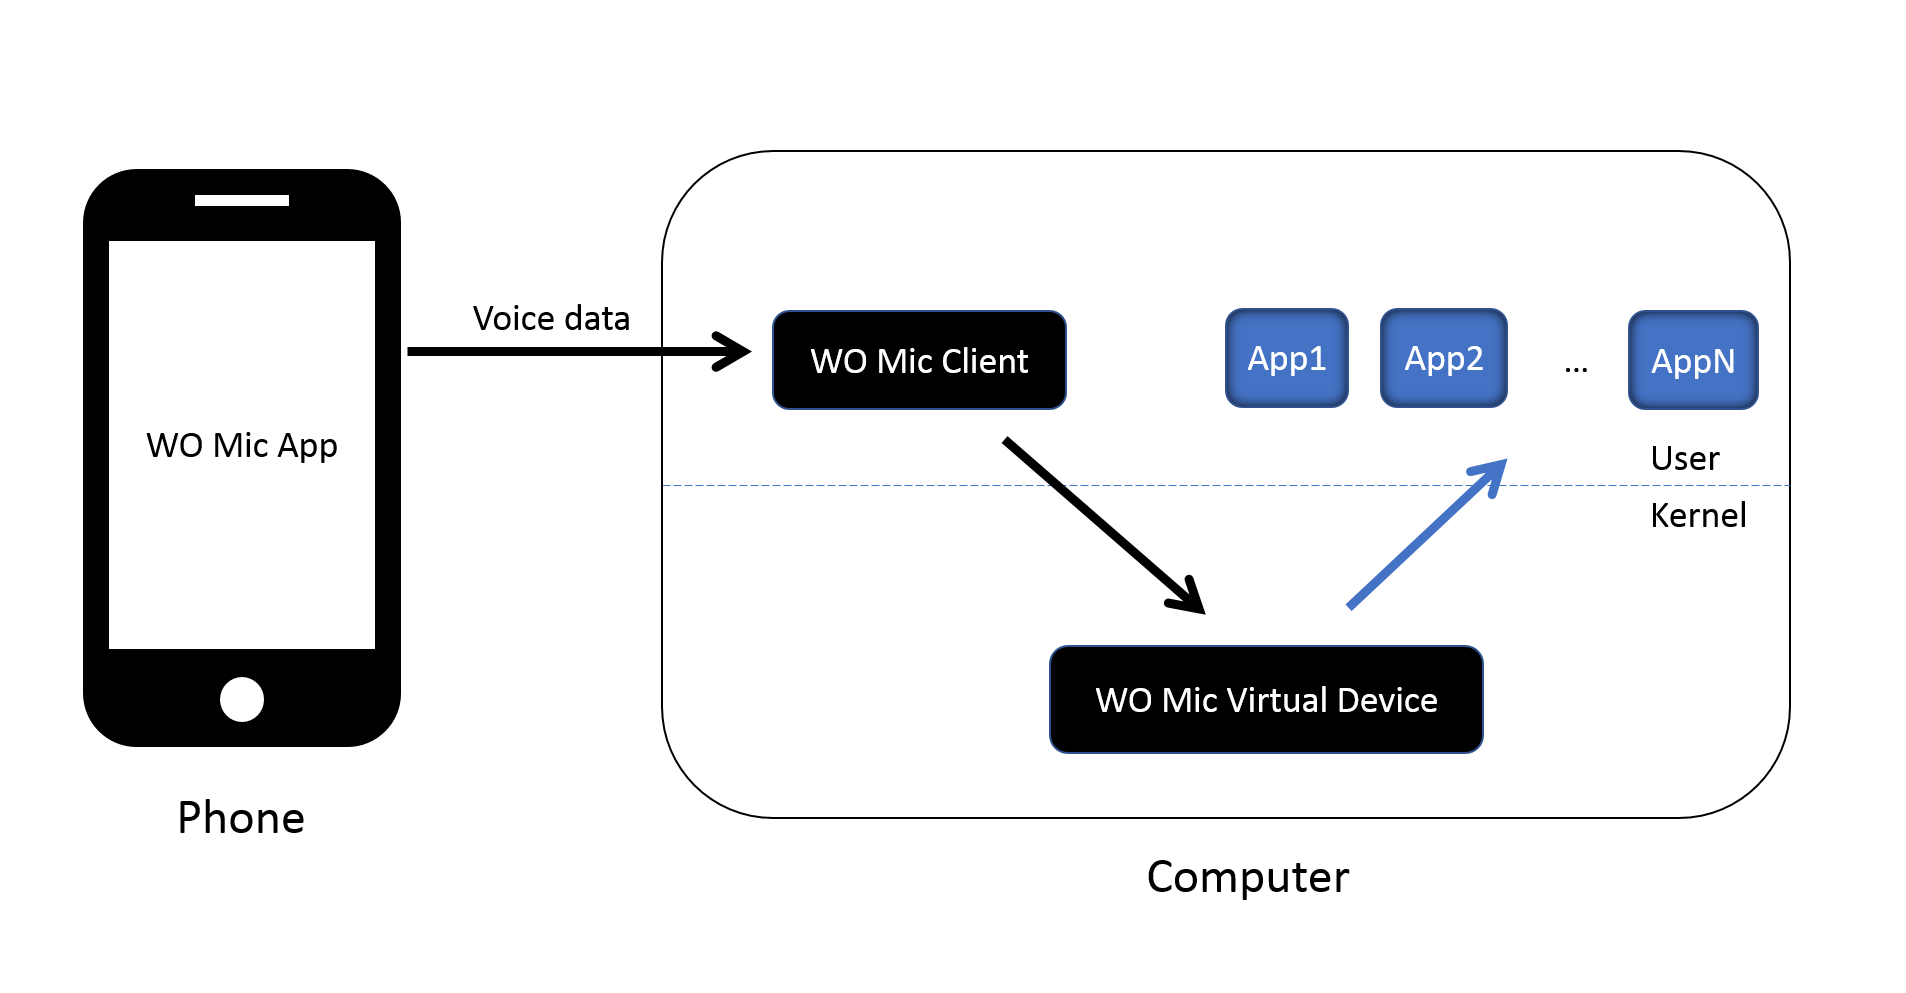
\includegraphics[width=0.65\textwidth]{Chapters/3CHP/Images/WOMICDiag.png}
    \caption{Physical connection of the phone microphone to the computer}
    \label{fig:MicConnectio}
\end{figure}
\subsection{Accelerometer}
As already mentioned in section \ref{sec:VibSens}, there are various types of accelerometers, however the choice of the one to use depends on various factors, for this particular application is important that the accelerometer in use has a low cost and a small size, for the future application. With this in mind the choice declines over MEMS accelerometers, that are smaller when compared with piezoelectric accelerometers.

The type of \acrshort{mems} accelerometers available is very wide, some of them started to be used in applications that usually uses piezoelectric accelerometers, like \acrshort{cbm}, \acrshort{shm}, \acrshort{ahm}, \acrshort{vsm} and \acrshort{iot}, for example. When selecting the accelerometer it is important to take into consideration some parameters, which are responsible to determine the category of the accelerometer, they are the application, the bandwidth and the range. Although there is no standard for the category on each accelerometer fits in, \textit{Analog Devices} has one document where they divide their products in different categories, with the type of application used in each on of them featuring a description of the key parameters that must be taken into consideration when selecting the appropriate accelerometer.
\begin{figure}[]
    \centering
    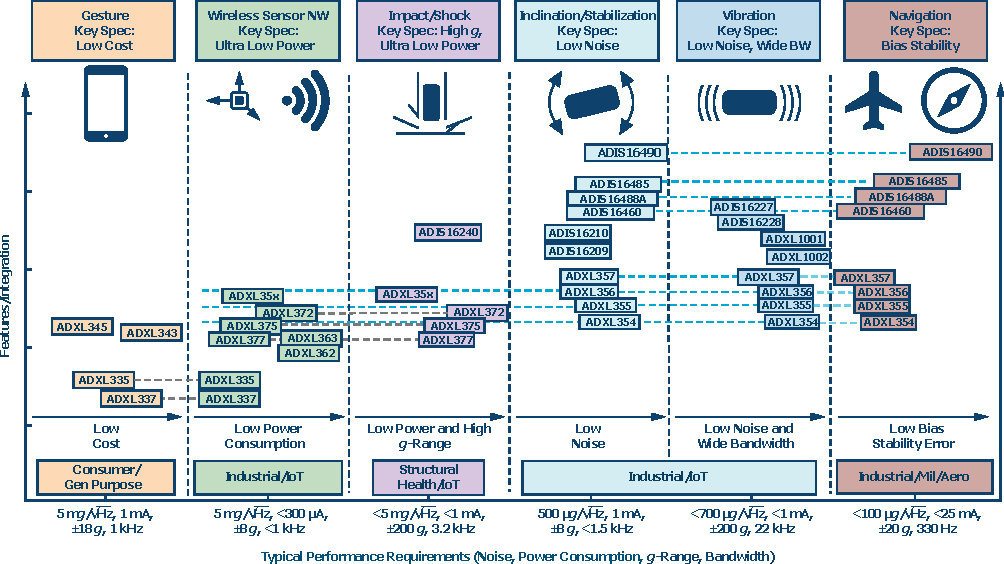
\includegraphics[width=1\textwidth]{Chapters/4CHP/Figures/adTable.pdf}
    \caption{Application landscape for a selection of Analog Devices MEMS accelerometers}
    \label{fig:adtable}
\end{figure}
The \acrshort{mems} accelerometers from \textit{Analog Devices} are divided in two families, the ADXLxxxx and the ADIS16xxxx, the last offers different advantages when compared with he first, more like a plug-and-play solution with features like factory compensation, embedded compensation and signal processing. This family obviously has one of the features that has particular interest for the application, in this case the fact that has signal processing on the accelerometer, on the other hand this comes with a price, and this family of products has a higher cost. So is necessary to define the key specifications of the accelerometer, in order to properly chose one\cite{AnalogDialogue51102017}\cite{AnalogDialogue51112017}.

The final purpose is to have a cheap and portable prototype, that is capable of accurately measuring the vibrations and determine the liquid level, this implies that his bandwidth covers the spectrum of frequency on which the curve of the relation liquid level vs frequency is. With this the key specifications are the low cost, low power and his bandwidth must close to 2kHz, determine as maximum frequency for a mechanical vibrations in \ref{tab:sampRat} and latter proved in the results obtained by \citeauthor{wuLiquidLevelDetector2014b} as described in \ref{sec:LPGModel}. Considering these specification, some models where chosen, that integrate this criteria, as follows:
\begin{table}
    \centering
    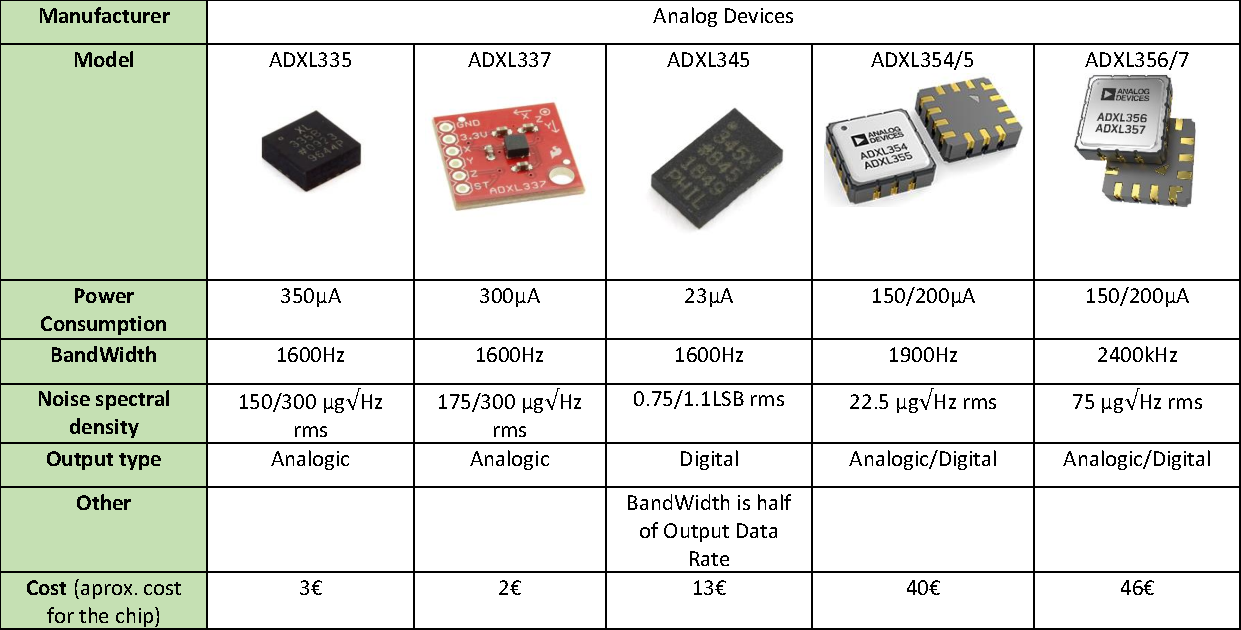
\includegraphics[width=1\textwidth]{Chapters/4CHP/Figures/accTable.pdf}
    \caption{Key specifications of MEMS accelerometers}
    \label{tab:acctable}
\end{table}
Although it doesn't accommodate entirely the specifications but since it was already available for use, the choice fell to the ADXL335. This model offers a low power consumption of around 350$\mu$A, his bandwidth is adjustable with a single capacitor per axis, from 0.5 to 1600 Hz for X and Y axis and 0.5 to 550Hz for Z axis. Beside this the accelerometer itself is very cheap, with a price starting at 3€. To properly acquire the data from this sensor and process it, is necessary to integrate it with an amplifier circuit and a microcontroller, on which more details will be explained further ahead.
\subsection{Piezoelectric}
%%Missing the images and the review
There are several types of piezoelectric constituents and a defining factor of the type of material used in the piezoelectric is the application. The most commonly used in vibration measurement is \acrshort{pvdf} as polymer and \acrshort{pzt} as ceramic. The reason for that is due the fact that they can measure either high or low frequencies. This sensor usually produces charges according to the applied pressure, the tension generated at the output is related with the amount of charges generated. In a electric point a view this is a sensor with a high-impedance, therefore is necessary a amplifier circuit with a high input impedance and with a high \acrshort{snr} relation. For piezoelectric it is usual to use a charge amplifier that already fills these requirements.

In the developed work, was used two different \acrshort{pzt} piezoelectric, with different dimensions, one with a diameter of 27mm and the other with a diameter of 12mm.

\begin{figure}[]
    \centering
    \begin{subfigure}{0.45\textwidth}
        \centering
        \includegraphics[width=\linewidth]{Chapters/4CHP/Figures/piezo27mm.png}
        \caption{}{}
        \label{subfig:piezo1}
    \end{subfigure}
    \begin{subfigure}{0.45\textwidth}
        \centering
        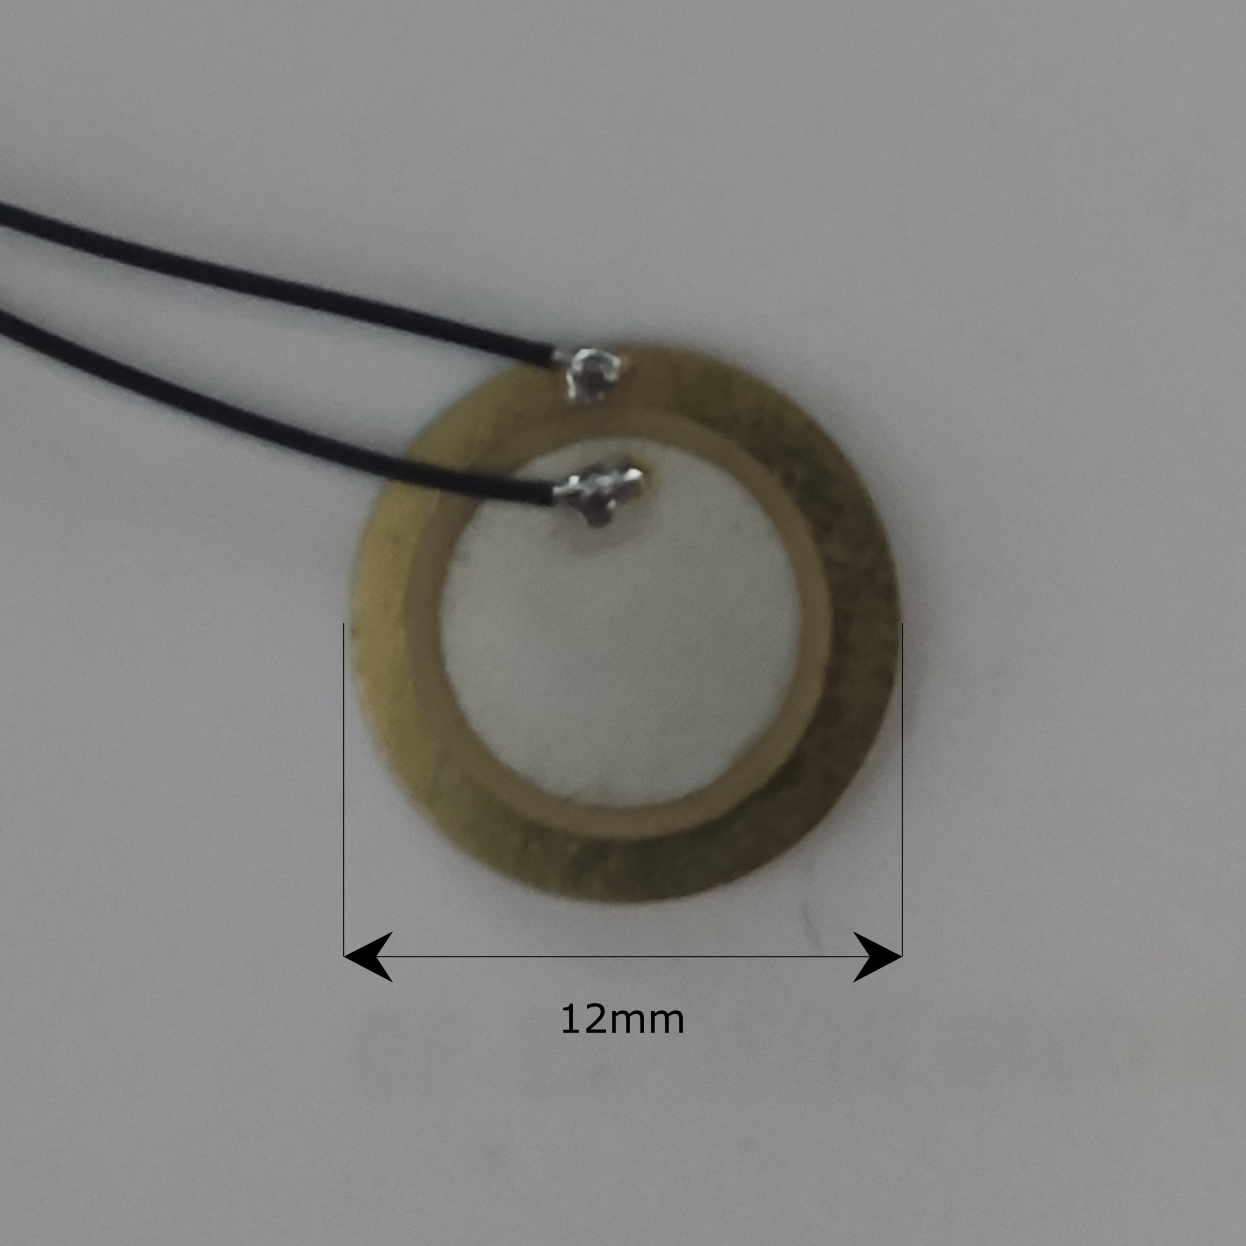
\includegraphics[width=\linewidth]{Chapters/4CHP/Figures/piezo12mm.png}
        \caption{}{}
        \label{subfig:piezo2}
    \end{subfigure}
    \caption{Piezoelectric sensors used}{}
    \label{fig:UsedPiezos}
\end{figure}
The use of a piezoelectric, is not only a cheaper option, when compared with the accelerometer, but also allows to pursue a different approach, is the desire to change from hitting the \acrshort{pzt} bottle to a different method of stimulation. 

\subsection{Microcontroller}
When selecting the microcontroller, it is important to have some specifications in mind, as in the perspective of a future implementation, one that is quite important is the performance, the cost, as well as the power consumption. There is a large variety of products that most certainly would fit in these specifications. The selection of this it took in consideration those characteristics and fell to one from Texas-Instruments, the model of the chosen microcontroller is the MSP-EXP430FR2433, his main characteristics are the following:
\begin{itemize}
    \item 16-bit \acrshort{risc} processor with a clock frequency up to 16MHz;
    \item 15KB of program and 512B information \acrshort{fram}, 4KB \acrshort{ram};
    \item 8-channel 10-bit \acrshort{adc};
    \item Four 16-bit Timers, 16-bit counter-only \acrshort{rtc};
    \item 32-bit Hardware-Multiplier;
    \item Two \acrshort{eusci}\_A, supports \acrshort{uart}, \acrshort{irda} and \acrshort{spi} and one \acrshort{eusci}\_B, supports \acrshort{spi} and \acrshort{i2c};
\end{itemize}
Beside these characteristics the microcontroller offers different low-power modes, that consume from hundreds of microAmps to a couple of hundreds of microAmps, depending on the mode of operation of the microcontroller. Another thing in consideration, when selecting, is the fact that it is possible to run with a super cap. The performance in this case is not as important as it seams, is not mandatory that operation that would need to be performed must return a liquid level to the user instantly, that means that the results not being in real time won't make much of a difference, anyway if that was the case, there is also a 32-bit Hardware-Multiplier embedded that reduces the use of \acrshort{cpu} time to perform multiplications that would be required\cite{MSP430FR2433DataSheet}. Associated with these characteristics, the price of this microcontroller is very appealing, starting under 2€.

\subsection{Solenoid}
For more constant measurement it is important that when the hitting process is constant as well, for that one a manual hammer is substituted by a solenoid, that when powered for a short period can simulate an impulse in the system. With that purpose was chosen the SOL01002, the reason is, first this solenoid work with tensions starting at 5V and the other reason is due the fact that is a Push type, which means that when powered the shaft will move and produce the impulse desire.
\begin{figure}[]
    \centering
    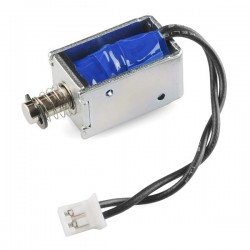
\includegraphics[width=0.45\textwidth]{Chapters/4CHP/Figures/solenoide.jpg}
    \caption{Solenoid used to stimulate the bottle}
    \label{fig:solenoid}
\end{figure}
The downside of using this model, can be the low impact force, it may not be able to produce a strong enough hit that can be detected by the sensors.
\section{Design}
\subsection{Accelerometer}

\subsection{Piezoelectric}
As mentioned, piezoelectric sensors can be used in many fields, for sensing acceleration, vibration, shock or pressure. To what is related to acceleration or vibration, the piezoelectric will output a charge that is a function of his deformation/deflection. For the application in specific, the vibration produce, although is noticeable directly at the piezoelectric output, has a small amplitude which means that needs to be amplified to allow a distinct difference between what is actually the vibration and the output of the piezoelectric itself, is important to properly design a signal conditioning amplifier circuit. Texas-Instruments has a very clear document explaining how to design charge amplifiers for piezoelectric sensors \cite{bartolomeSignalConditioningPiezoelectric2010}, on which they clearly explain different types of circuit for this application in specific, with the advantages and disadvantages. The simplest model of this type of circuit is as follows: 
\begin{figure}[]
    \centering
    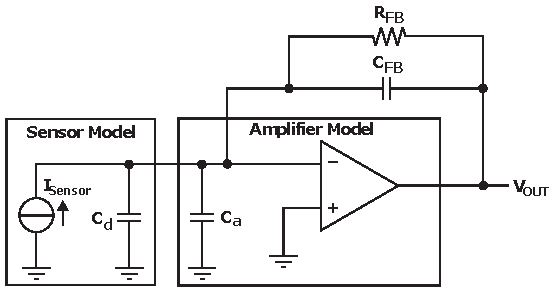
\includegraphics[width=0.45\textwidth]{Chapters/4CHP/Figures/singleenddedchargeamp.pdf}
    \caption{Charge Amplifier for signal conditioning}
    \label{fig:ChargeAmpSimp}
\end{figure}
Two important things to consider is the bandwidth and the gain of the circuit. In the first case, the circuit functions as a High-Pass Filter which means that when selecting the feedback resistor and capacitance, their values must be selected to keep a low pole in the filter.
\begin{equation}\label{eq:fhpf}
    f_{HPF} = \frac{1}{2\pi R_{FB}C_{FB}}
\end{equation}
Usually the value of the resistor in use is on the order of hundred of megaohms and the capacitance should be low, the reason is due to the fact that in these circuits the gain is defined by the value of the capacitance, the lower is value, the higher the gain.
\begin{equation}
    Gain = \frac{1}{C_{FB}} (mV/C)
\end{equation}
Another factor that must be taken in consideration is the \acrshort{snr}, this value needs to be maximized. For this circuit in specific, one way to archive this is by increasing the value of $R_{FB}$ as much as possible. To outline this and improve the \acrshort{snr} value is through the use of a differential charge amplifier.
\begin{figure}[]
    \centering
    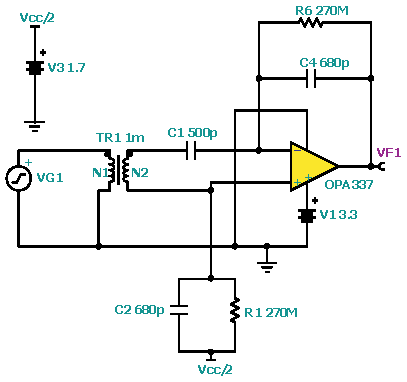
\includegraphics[width=0.45\textwidth]{Chapters/4CHP/Figures/differentialchargeamp.pdf}
    \caption{Differential Charge Amplifier for signal conditioning}
    \label{fig:ChargeAmpDif}
\end{figure}
This circuit offers two main advantages when compared with a simple charge amplifier, the first is related with the gain, in this case has twice the gain of a single-ended input circuit, (while the noise increases only as a square-root function???). The second is due to the fact that these circuits are very sensitive, in a single-ended input one of the terminals injects current while the other is connected to the ground, this will amplify the interference. In a differential input the common-mode signals will cancel each other.

For the practical application, the  circuit in use will be as shown in figure \ref{fig:ChargeAmpDif}, considering the simulation that the document \cite{bartolomeSignalConditioningPiezoelectric2010} presents, mainly those related with the \acrshort{snr}, this seemed to be the suitable choice for the application, since noise is a key aspect when measuring the signal, this is one way of reducing the effect of it. The difference in the circuit in use will be the components, the \acrshort{opamp} in use will be the MCP602 from MicroChip, as for the remaining components, if is consider the information from the document, it can be select the values of 1nF for the capacitors and 100M$\Omega$ for the resistors. With these values the pole of the High-Pass Filter will be set at 1,59Hz and the gain of the circuit 2G(mV/C).
\begin{figure}[]
    \centering
    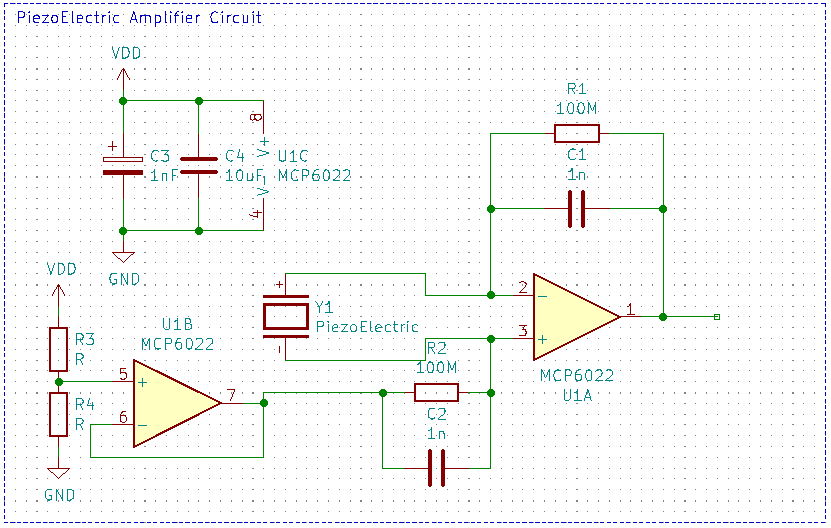
\includegraphics[width=0.45\textwidth]{Chapters/4CHP/Figures/piezoAmpcirc.PNG}
    \caption{Differential Charge Amplifier Schematic}
    \label{fig:ChargeAmpDifSCH}
\end{figure}
Note that,once again, beside being connected in differential mode, the circuit has on its positive input fixed input voltage of half the supply voltage of the OpAmp.
\subsection{Solenoid}
The circuit needed for driving a solenoid is very simple, it consists simply in a \acrshort{mosfet}, a diode and a resistor as components. Is needed to pay attention to the used \acrshort{mosfet}, if the solenoid is active by a microcontroller, that in a high output has 3.3V in the specified pin, is needed to be one with a threshold voltage from the gate to the source. The use of the diode in parallel with the solenoid is to forward the current when the \acrshort{mosfet} is switched off. In figure \ref{fig:solenoidshc} is the schematic of the circuit used to drive the solenoid.
\begin{figure}[]
    \centering
    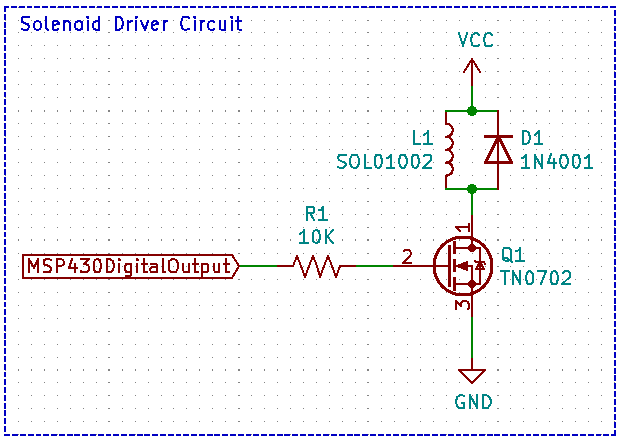
\includegraphics[width=0.65\textwidth]{Chapters/4CHP/Figures/SolenoidDriver.PNG}
    \caption{Circuit for driving the solenoid}
    \label{fig:solenoidshc}
\end{figure}
\section{Capture/Coupling}
\subsection{Microphone}
To position the microphone and acquire the sound produced when hitting the tank surface, the microphone was placed perpendicular to the surface of the tank and as close as possible from it, is also recommended to place it near the hitting point. With caution not to hit the microphone while measuring. The figure \ref{fig:micmount} is an illustration of how the microphone is placed relative to the \acrshort{lpg} bottle.
\begin{figure}[]
    \centering
    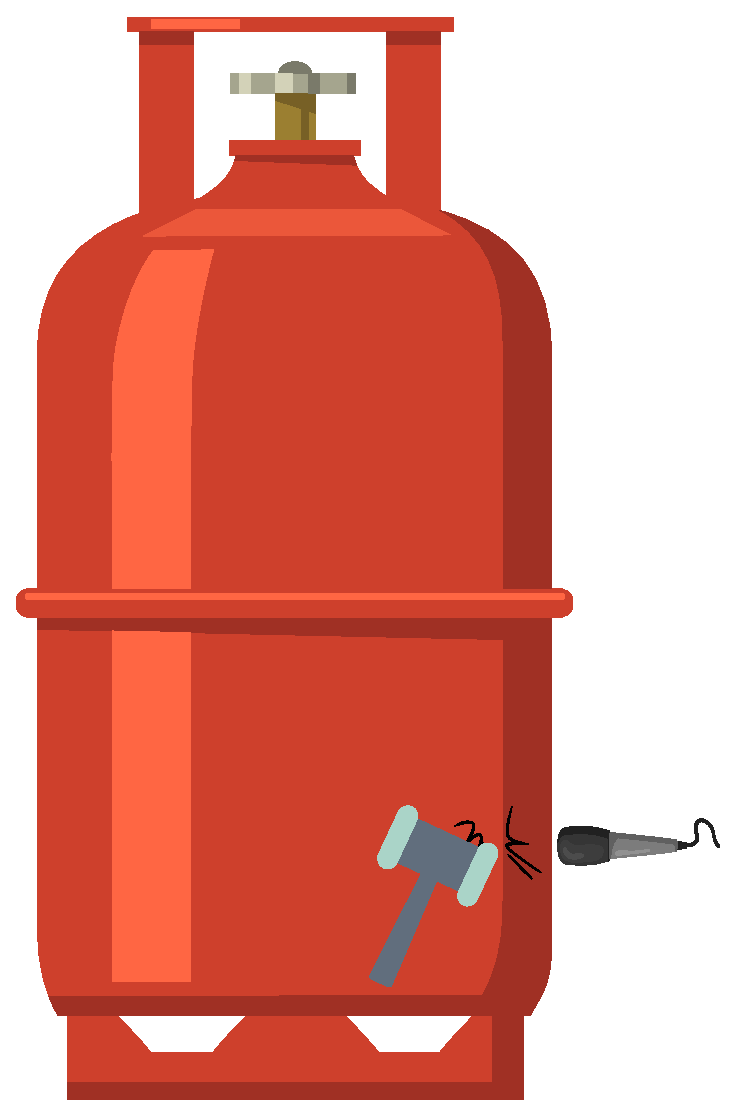
\includegraphics[width=0.3\textwidth]{Chapters/4CHP/Figures/micWimpactHamm.eps}
    \caption{Illustration of the accelerometer mount with a load strap}
    \label{fig:micmount}
\end{figure}
In the practical setup, since it uses the microphone from the phone, the side of the phone where the microphone is, should be faced to the \acrshort{lpg} bottle, usually the bottom part.
\subsection{Accelerometer}
When using an accelerometer for sensing vibration, there are different methods to mount it to the surface desired to measure those vibrations. Usually in the industry the accelerometer is mounted to the surface with a screw, allowing a great contact with the surface, but in the application pretended is not possible to use that method since that would imply the change in the structure of the tank and the accelerometer in use is not ready for a screw mount, anyway there are other methods to attach the accelerometer to the tank and even though that the examples from \cite{GuidelinesMountingTest} are to accelerometers with a screw mount, their examples can easily adapted to the type of accelerometer in use without any changes in the structure.

The type of mount is quite important in the frequency response of the accelerometer as well as the surface on which the accelerometer is going to be mounted at. The best results are usually obtained with a stud or screw mount, but that isn't possible since it would require structural changes to the tank, two other options are presented. One of the option is by using an adhesive, this is a possibility, but in a practical mount the surface and the sensor would require different mounting bases, to avoid damaging the sensor and allow to the sensor to be removed any time that is required, although this is practical to mount would also require that each tank had already the adhesive for the mount. When compared with the other two methods to mount, this offers worse frequency response accuracy. The second option is a magnetic mount, although as a lower frequency accuracy when the first two methods, stud and screw, this method offers a convenient mount if the structure of the tank is metallic, for this case is advised that the magnet is in a separate piece, to avoid damaging the accelerometer, magnets with a high pull strengths are better in providing a good frequency response, a system with dual-rail mount is god when the surface that the sensor is mounted on, is curve, but this decreases the operational frequency range of the accelerometer.

For the mount of the accelerometer in the \acrshort{lpg} bottle, will be used a magnet mount, is the most practical mount for a future application. Although in a laboratory environment and for test effects it won't be the only type of mount used. The first mount method will be with a load strap, this will hold firmly the sensor against the wall of the tank, as will be used for the first tests. In figure \ref{fig:mounLoadStrap} is an illustration of the sensor mount.
\begin{figure}[]
    \centering
    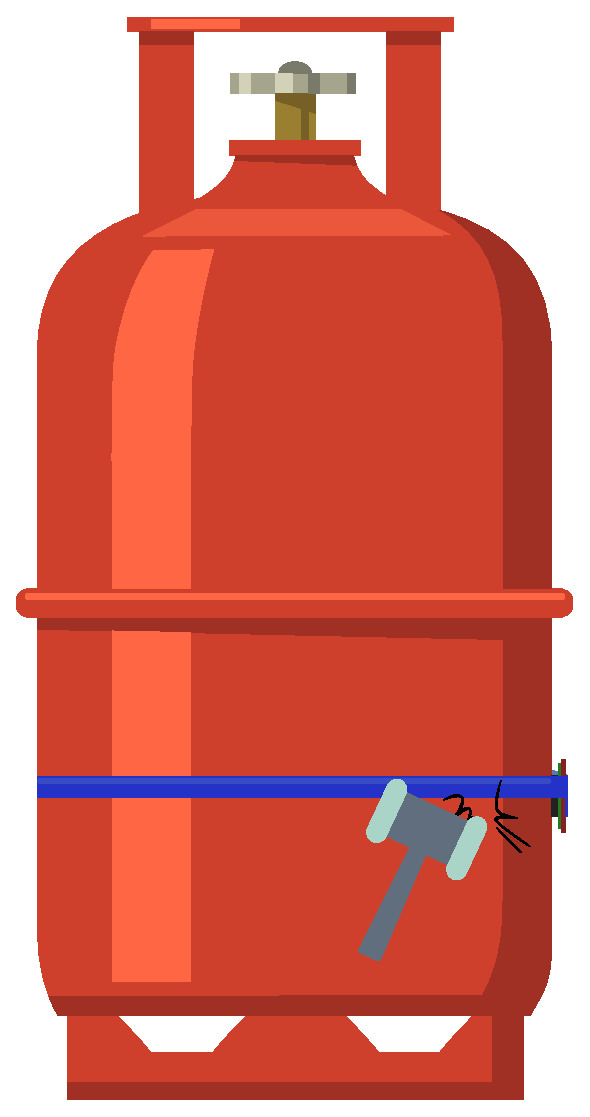
\includegraphics[width=0.3\textwidth]{Chapters/4CHP/Figures/AccLoadStrap.eps}
    \caption{Illustration of the accelerometer mount with a load strap}
    \label{fig:mounLoadStrap}
\end{figure}
For the magnet mount, there are actually two proposals, if by any reason one doesn't produce any results. In figure \ref{fig:mounMagnet} [a] is the ideal option, since it is less invasive for the accelerometer, for the reason mentioned above. In this case, a piece is design to be able to mount with two neodymium magnets at the top and bottom of the piece, this will pull the piece against the wall of the tank, between the two magnets is the necessary space for held the accelerometer, a sponge will be glued to the piece on one side and the other will be glued to the accelerometer, this will be slightly thicker than the piece, that way when the magnets attached the piece against the tank wall, the sponge will be compressed and and the surface of the accelerometer is expected to be firmly held against the tank wall as well. In figure \ref{fig:mounMagnet} [b], the mount is not ideal, since the neodymium magnet will be glued to the accelerometer surface for a god contact, this may result in best results when compared with the first option, but can damage the accelerometer, when attaching or removing the accelerometer from the tank wall.
\begin{figure}[]
    \centering
    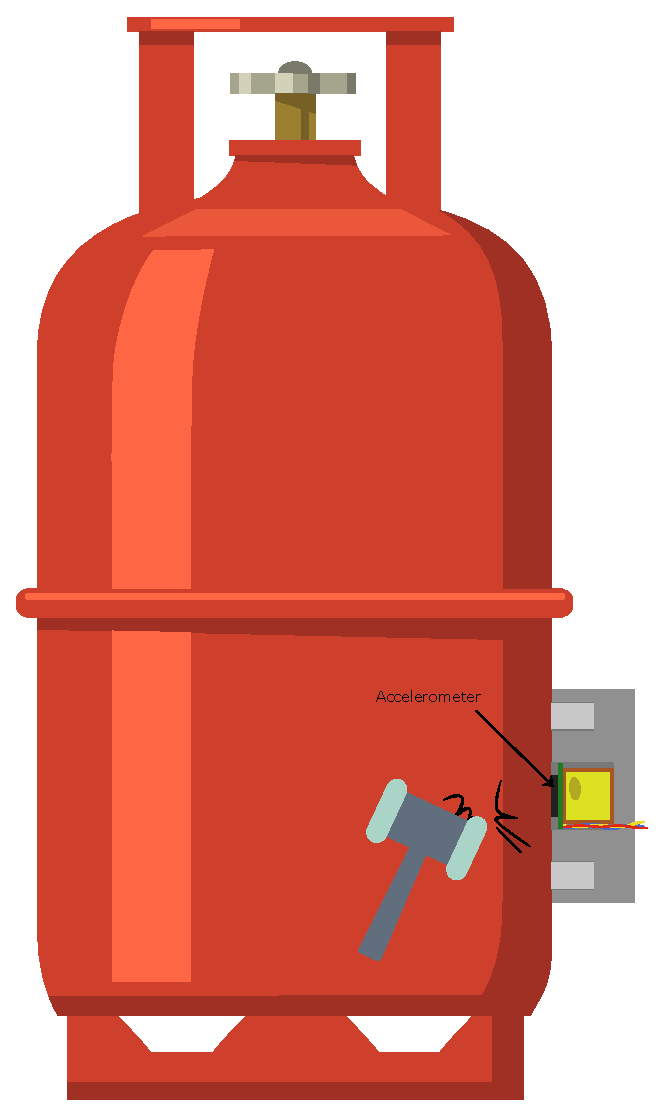
\includegraphics[width=0.3\textwidth]{Chapters/4CHP/Figures/AccMagnets.eps}
    \caption{Illustration of the accelerometer mount with magnets}
    \label{fig:mounMagnet}
\end{figure}
%

\subsection{Piezoelectric}
When mounting piezoelectric sensors, there is some considerations to take into account, the considerations are as well related with the application of the sensor. \acrshort{ti} provides a document with considerations for mounting a piezoelectric sensor to measure liquid level using ultrasonic waves, although is a different approach, the key aspect for mounting this type of sensors can be used as well to define how to properly mount them. What needs to be taken into account, according to the document is if the sensors is to be mounted inside or outside, at the top or at the bottom and for last the temperature range that the sensor can handles before starts to degrading the piezoelectric capability, it is quite clear the first aspect, since is suppose to be a non-invasive solution, which means that should be places at outside of the tank, the second aspect is not relevant since is being measured the vibration, not being used ultrasound to measure the liquid limit where the wave is reflected, the third aspect is also not that important since is expected to have the sensor at environment temperature unless, and this can be seen as an exception, when the gas from the tank has been release for a long period causing the outer wall of the bottle to freeze. Beside the first, which was already a requirement, none of the others will have a significant difference. For the purpose of measure trough the walls of the tank is required to have a good contact between the transducer and the mounting surface, in their application the glue the transducer directly to the surface of the tank \cite{minasiHowSelectMount2015}.

Since the application isn't ideal to have the transducer glued to the surface, the approach to have a good contact will be different, although the good results aren't guaranteed. The figure \ref{fig:coupPiezo} is the illustration of two different mounting pieces for the transducer.
\begin{figure}[]
    \centering
    \begin{subfigure}{0.3\textwidth}
        \centering
        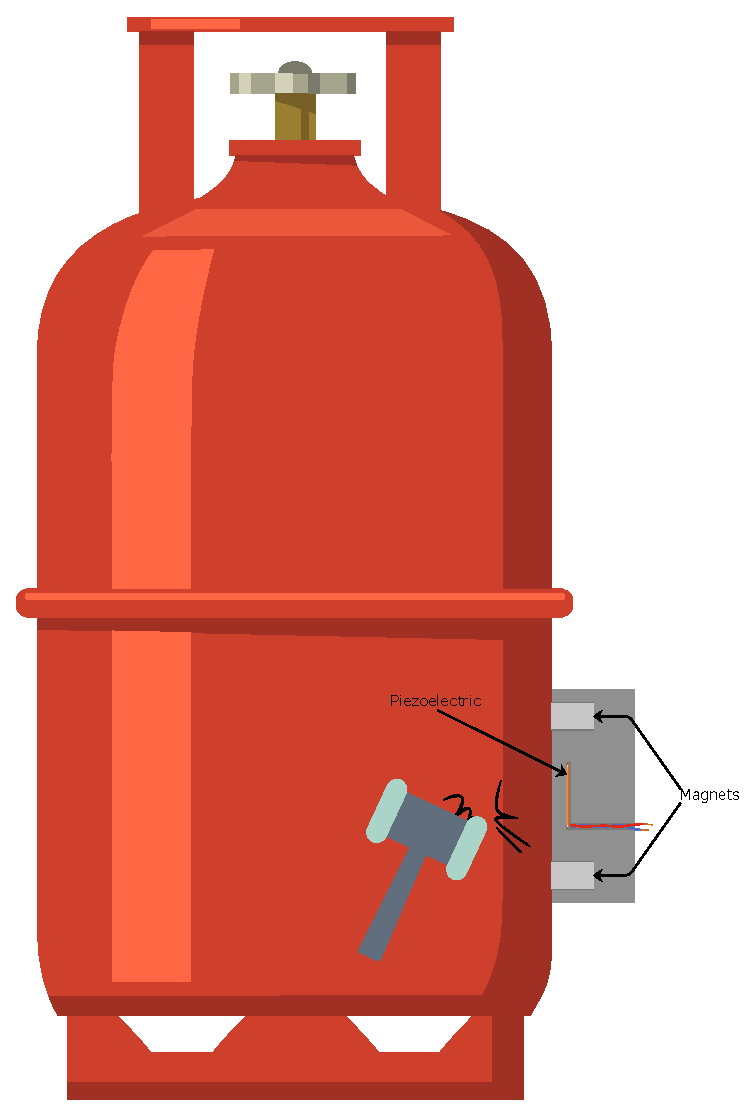
\includegraphics[width=\linewidth]{Chapters/4CHP/Figures/PiezoMagnetsSlot.eps}
        \caption{}{}
        \label{subfig:piezoslot}
    \end{subfigure}
    \begin{subfigure}{0.3\textwidth}
        \centering
        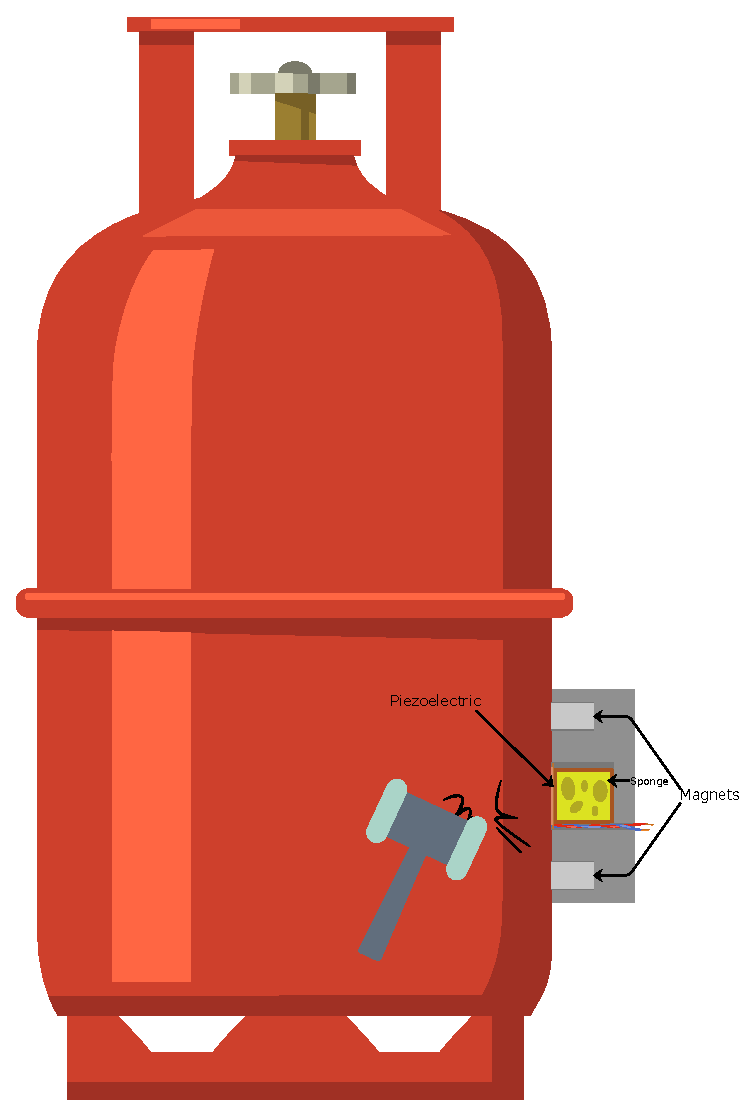
\includegraphics[width=\linewidth]{Chapters/4CHP/Figures/PiezoMagnets.eps}
        \caption{}{}
        \label{subfig:piezosponge}
    \end{subfigure}
    \caption{Illustration of the piezoelectric mount with magnets}{}
    \label{fig:coupPiezo}
\end{figure}
Both pieces will stay held to the tank with two neodymium magnets, one at the top of the piece and the other at the bottom. In figure \ref{fig:coupPiezo}~\subref{subfig:piezoslot}, the transducer is embedded in the piece, there is a slot in the middle, when the entire piece vibrates, the transducer vibrates with it, in the figure \ref{fig:coupPiezo}~\subref{subfig:piezosponge}, the coupling of the transducer is different when compared with the first one presented, the transducer id held glued to a sponge, and the sponge to the piece, the sponge is larger than the hole that is glued in the piece so when the entire piece is attached to the walls of the tank with the help of the neodymium magnets, it guarantees a god contact of the transducer with the wall since the sponge will press it against the wall and when there is vibration in the wall of the tank, is expected to the transducer to capture the actual vibration. 
\section{Extras - Delete later}
%\begin{gather}
%    \Delta_{10} = \frac{1-0}{2^{10}} \approx 0.98\cdot10^{-3}\\
%    \Delta_{8} = \frac{1-0}{2^{8}} \approx 3.9\cdot10^{-3}
%\end{gather}

%\begin{equation} \label{eq:maxf}
%    f_{Max} = \frac{1}{T-WNS} = \frac{1}{10\cdot 10^{-9} - 0.188\cdot 10^{-9}} = 101.9\,MHz
%\end{equation}

%\begin{itemize}
%    \item \textbf{AXI4} implements a highly customizable memory mapped interface, indicated for complex applications;
%    \item \textbf{AXI4-Lite} is a simplified version of the former, keeping the memory mapped communications;
%    \item \textbf{AXI4-Stream} implements a streaming protocol, allowing a high throughput.
%\end{itemize}

%\begin{figure}[!htb]
%    \centering
%    \includegraphics[width=\textwidth]{Sections/4DevelopedArchitecture/Figures/DCTCop.png}
%    \caption{Block design generated by \emph{Vivado} for integration of \emph{DCT Wrapper} with \emph{Microblaze}.}
%    \label{fig:blockdes}
%\end{figure}

%\begin{table}[!htpb]
%    \centering
%    \caption{Add Caption}
%    \begin{tabular}{ccccc} \toprule
%        {}&{}&{}&{}&{}\\
%        \bottomrule
%    \end{tabular}    
    %\label{tab:maxfps}
%\end{table}


\clearpage
%\printbibliography[heading=subbibliography]
%\addcontentsline{toc}{section}{References}